% Auto-generated by scripts/07_figures.py. Requires \usepackage{graphicx}.

\begin{figure*}[t]
  \centering
  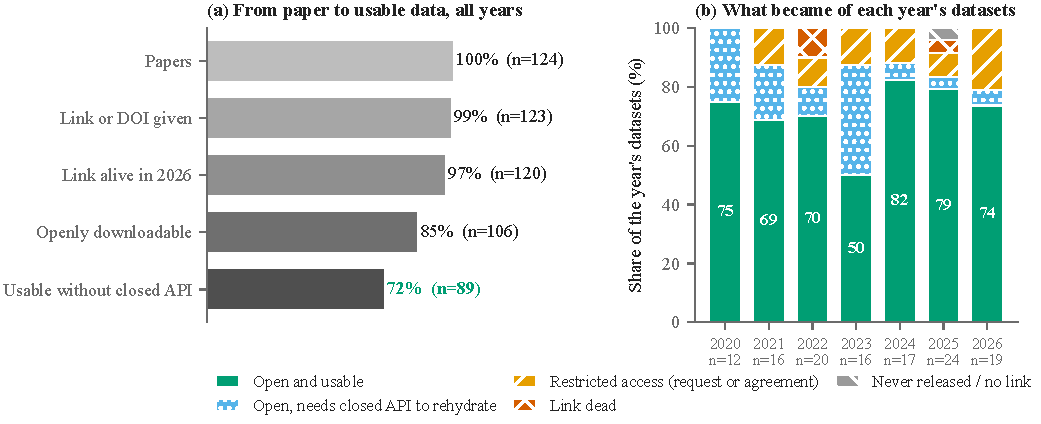
\includegraphics[width=\textwidth]{figures/fig1_funnel_and_fate.pdf}
  \caption{Available is not usable. (a) Of all ICWSM Dataset Track papers, the share that clears each step from a claimed release to data a researcher can actually use in 2026. (b) The 2026 state of every dataset, by publication year; the number on each bar is the share that is openly usable.}
  \label{fig:funnel_and_fate}
\end{figure*}

\begin{figure*}[t]
  \centering
  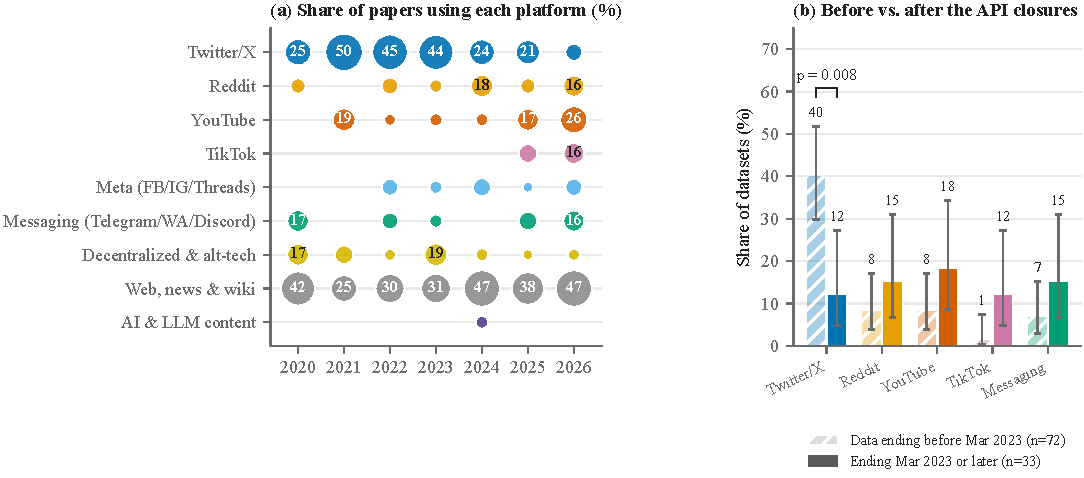
\includegraphics[width=\textwidth]{figures/fig2_platform_migration.pdf}
  \caption{Platform migration. (a) Share of each year's dataset papers that include each platform family (bubble area proportional to share). (b) Share of datasets including each platform, split by when data collection ended: before or after March 2023, when free Twitter/X API access ended (followed by Pushshift, free Reddit API access and CrowdTangle). Error bars are 95\% Wilson intervals; p from a chi-square test.}
  \label{fig:platform_migration}
\end{figure*}

\begin{figure}[t]
  \centering
  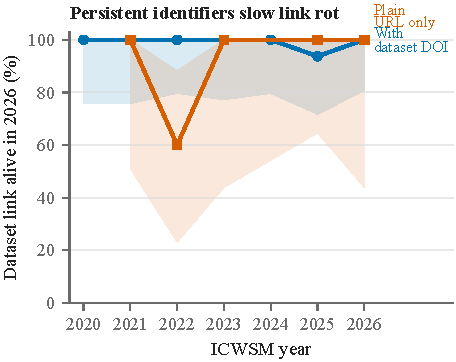
\includegraphics[width=\columnwidth]{figures/fig3_link_survival.pdf}
  \caption{Share of dataset links that still resolve in 2026, by publication year, for datasets with and without a dataset DOI. Ribbons are 95\% Wilson intervals; cohorts with fewer than three papers are omitted.}
  \label{fig:link_survival}
\end{figure}

\begin{figure}[t]
  \centering
  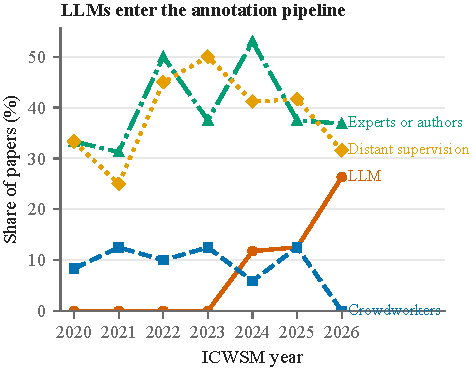
\includegraphics[width=\columnwidth]{figures/fig4_annotation_shift.pdf}
  \caption{Share of dataset papers using each source of labels (papers can use several). LLM includes pipelines where humans verify or correct LLM labels.}
  \label{fig:annotation_shift}
\end{figure}

\begin{figure}[t]
  \centering
  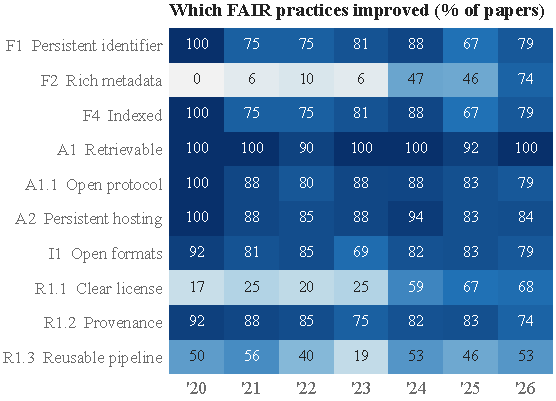
\includegraphics[width=\columnwidth]{figures/fig5_fair_heatmap.pdf}
  \caption{Share of papers meeting each operational FAIR indicator, by year. Indicators combine what papers report with what the 2026 audit observed (definitions in Table~\ref{tab:fair}).}
  \label{fig:fair_heatmap}
\end{figure}

\begin{figure}[t]
  \centering
  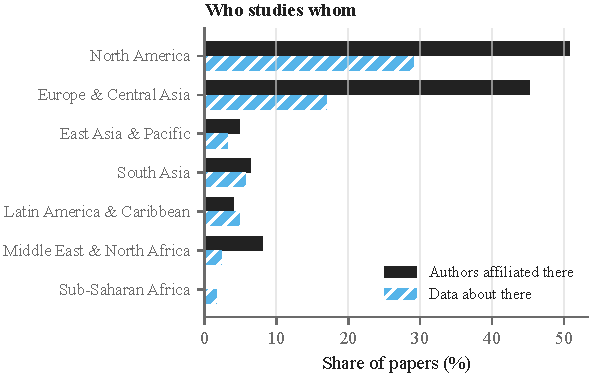
\includegraphics[width=\columnwidth]{figures/fig6_who_studies_whom.pdf}
  \caption{Share of papers with at least one author affiliated in each world region, compared with the share whose data is about that region. Gaps show regions studied mostly from elsewhere.}
  \label{fig:who_studies_whom}
\end{figure}

\begin{figure}[t]
  \centering
  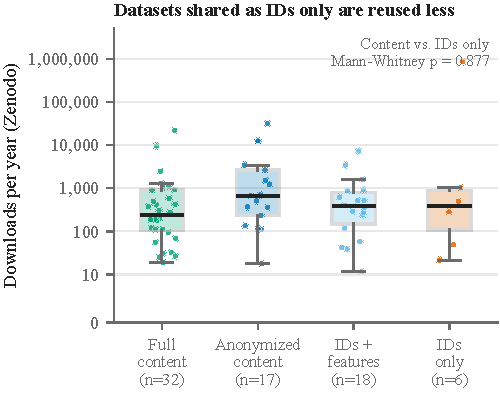
\includegraphics[width=\columnwidth]{figures/fig7_reuse_by_release_form.pdf}
  \caption{Age-normalized annual downloads by release form, restricted to Zenodo so that every dataset is measured with the same counter (symlog scale). Download counters are not comparable across repositories.}
  \label{fig:reuse_by_release_form}
\end{figure}

\begin{figure*}[t]
  \centering
  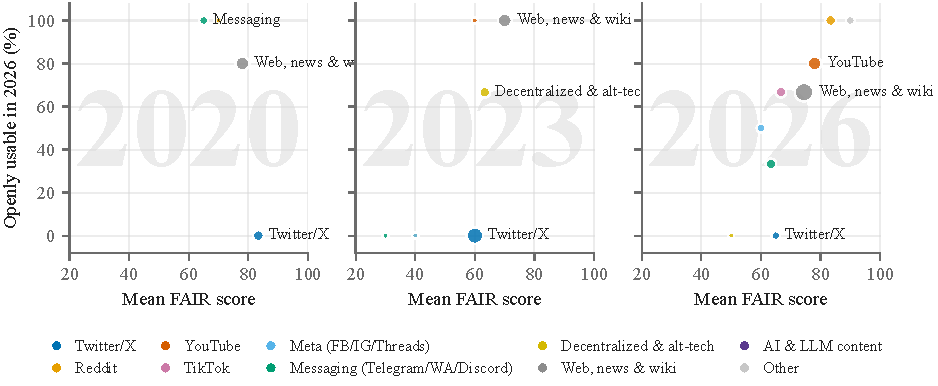
\includegraphics[width=\textwidth]{figures/fig8_gapminder_snapshots.pdf}
  \caption{Platform families as bubbles, in the style of Gapminder. Horizontal position: mean FAIR score of that family's datasets; vertical: share still openly usable in 2026; area: number of datasets that year. Younger cohorts have had less time to decay, so compare bubbles within a panel, and movement between panels. An animated version is in the repository and the web explorer.}
  \label{fig:gapminder_snapshots}
\end{figure*}

\begin{figure}[t]
  \centering
  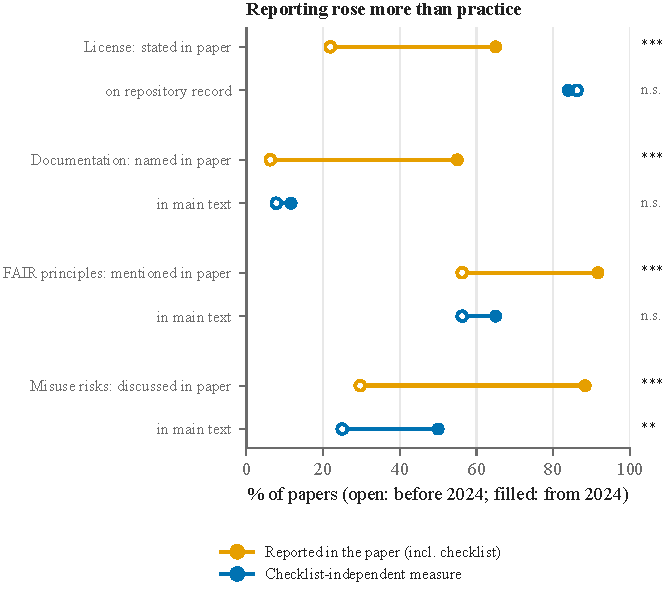
\includegraphics[width=\columnwidth]{figures/fig9_talk_vs_practice.pdf}
  \caption{Papers before and after the ICWSM paper checklist (2024). Orange: the practice as reported anywhere in the paper, including checklist answers. Blue: an independent measure of the same practice, namely the license recorded on the repository record, or mentions in the main text before the references. Fisher's exact test: * p<0.05, ** p<0.01, *** p<0.001.}
  \label{fig:talk_vs_practice}
\end{figure}
